\section{Temporal Graph Model}
\label{sec:tga}

\begin{figure}[t]
\centering
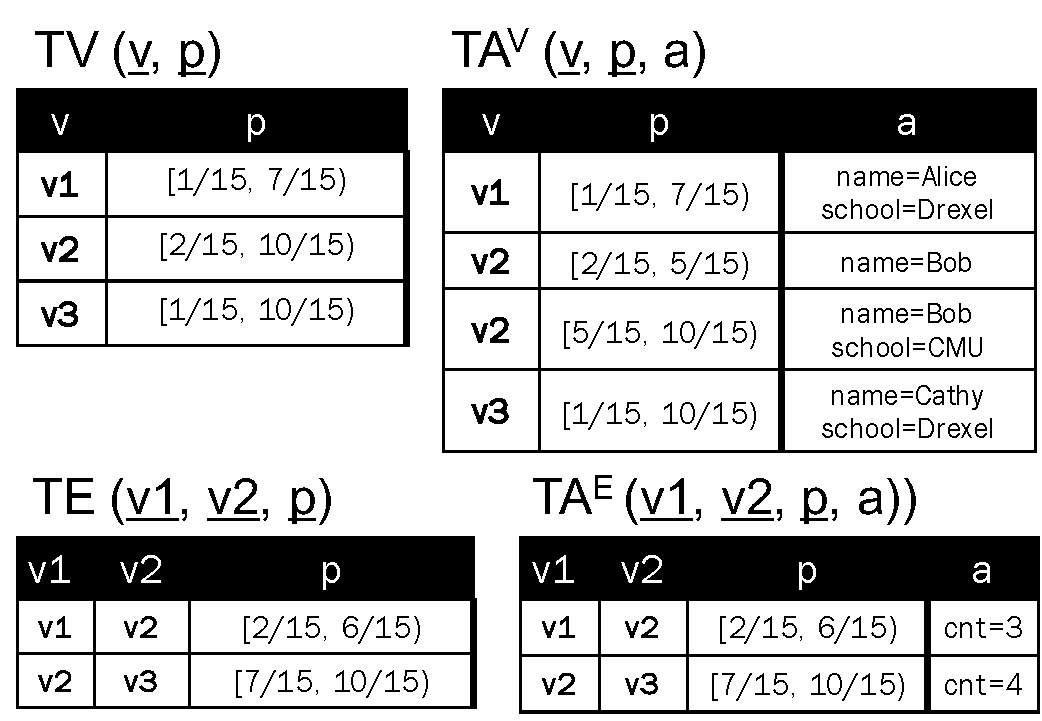
\includegraphics[width=3in]{figs/T1_rel.pdf}
\vspace{-0.2cm}
\caption{\tg \insql{T1}.}
\vspace{-0.4cm}
\label{fig:tg_rel}
\end{figure}

{\bf Data model.}  In~\cite{PortalarXiv2016} we proposed an evolving
graph model \tg based on temporal relations with point semantics.
Briefly, an evolving graph consists of two temporal relations, V and
E, which represent the vertices and edges of the graph with their
corresponding periods of validity expressed by intervals.
Optionally, two other relations VA and EA represent the vertex and
edge attributes using the property model, also with their periods of
validity.  An example is shown in Figure~\ref{fig:tg_rel}.

A \tg represents a single graph, and models evolution of its topology
and of vertex and edge attributes.  A snapshot of the graph is the
state of the relations at any time point.  Relations of \tg are
coalesced~\cite{DBLP:conf/vldb/BohlenSS96} --- each fact (existence of
a vertex or edge, or an assignment of a value to a vertex or edge
attribute) is represented exactly once for each time period of maximal
length during which it holds.  We also require that referential
integrity holds on E w.r.t. V, on VA w.r.t. V, and on EA w.r.t. E,
guaranteeing that edges only exist if their end points exist at the
same time, and similarly for vertex and edge attributes.

{\bf Operations.} In~\cite{PortalarXiv2016} we also proposed a
temporal graph algebra \tga.\eat{ which is vertex- and edge-complete
  in relation to the temporal relational algebra. } \tga is
compositional: operators take a \tg or a pair of \tgs as input, and
output a \tg.  \tga semantics can be expressed as a sequence of
temporal relational algebra expressions, guaranteeing snapshot
reducibility and extended snapshot
reducibility~\cite{DBLP:reference/db/Bohlen092} --- two properties
that are appropriate for a point-based temporal data model.  We study
the expressiveness of \tga and show completeness with respect to
temporal relational algebra (TRA).

The \tga operations include slice, map, selection, aggregation, node
creation, edge creation, and common set operators union, intersection,
and difference.  We explain some of these operations in the next
section through examples.  We also support Pregel-style analytics that
are logically executed on each snapshot.

